\subsection{Task}

\begin{frame}{Single-Document, Sentence-Extractive Summarization}
    \begin{columns}
        \begin{column}{0.5\textwidth}
            \textbf{Text Unit:} Sentence\\
            \vspace{10pt}
            \textbf{Input:} A sequence of sentences, $s_1,\ldots, s_n$\\
            \vspace{10pt}
            \textbf{Output:} A sequence of binary extraction predictions, $y_1, \ldots, y_n$
        \end{column}
    \begin{column}{0.5\textwidth}
        \begin{center}
            \resizebox{\textwidth}{!}{\begin{tikzpicture}[
                sent/.style={font=\large,anchor=north west, align=left},
                    ]
            \node<1-2>[inner sep=0pt] (bg) at (0,0)
            {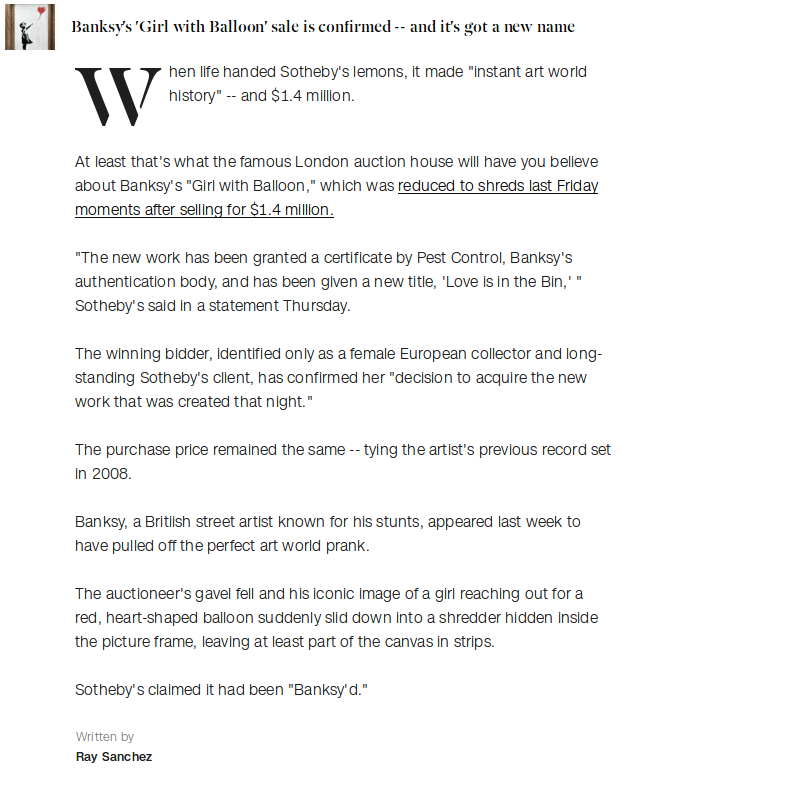
\includegraphics[width=.90\textwidth]{images/ext/article_before.png}};
            \node<3>[inner sep=0pt] (bg) at (0,0)
            {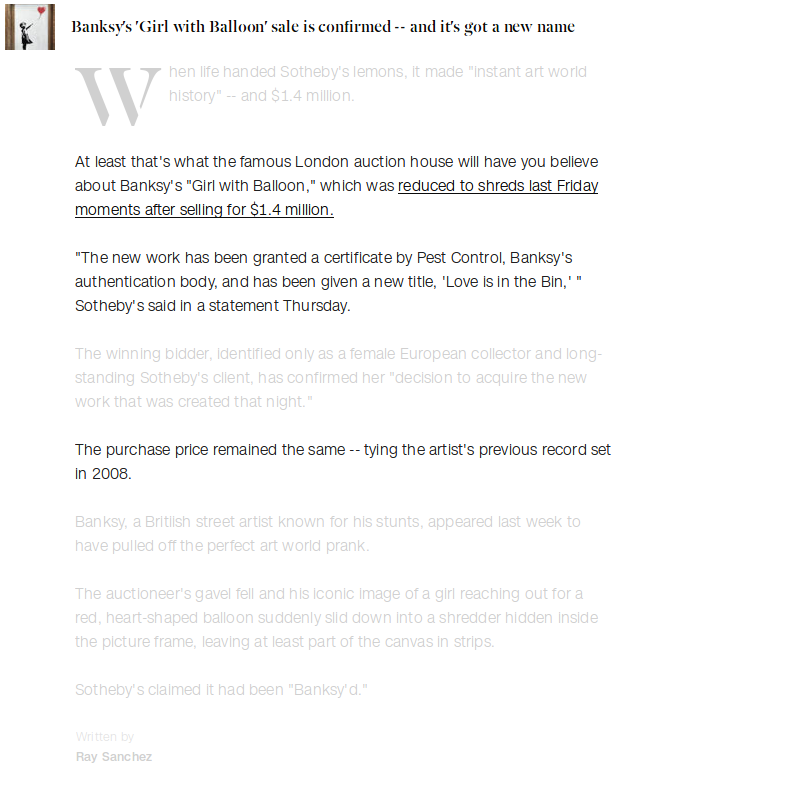
\includegraphics[width=.90\textwidth]{images/ext/article_after.png}};

    \foreach \y/\px [count=\yi] in {0/2.8,1/2.0,1/1.3,0/0.5,1/-0.2,0/-0.8,0/-1.5,0/-2.1}  {
        \node[sent] (s\yi) at (1.5,\px ) {$\uncover<2->{\rightarrow y_\yi}\uncover<3->{=\y}$};
        \node[sent] (s\yi) at (-3.55,\px ) {$s_\yi=$};
    }
    \end{tikzpicture}}
  \end{center}
  \end{column}
  \end{columns}
\end{frame}

\begin{frame}{Deep learning for Extractive Summarization}

  \begin{itemize}
    \item Lots of recent research activity using deep learning for
              summarization!  \\~\\
              
            \begin{center}$\underbrace{p(y_1,\ldots,y_n|s_1,\ldots,s_n;\theta)}_{\text{neural model with parameters $\theta$}}=\prod_{i=1}^n \underbrace{p(y_i|y_{<i},s_1,\ldots,s_n;\theta)}_{\text{salience of $s_i$}}$ \end{center}

              ~\\
              ~\\
    \item Unclear what model design choices are most effective.\\
              \uncover<2>{\alert<2>{We perform a comparison of some task specific
              architectures to simplified or ``standard'' models.\\}}
              ~\\
    \item Unclear what are the most important signals in the data for
              learning.\\
              \uncover<2>{\alert<2>{We perform a several ablation experiments
              to understand the contributions of lexical semantics vs.
              structure/discourse.}}
  \end{itemize}

\end{frame}


